\documentclass[aspectratio=169,14pt]{beamer}

\usepackage{graphicx}
\usepackage{booktabs}
\usepackage{amsmath}
\usepackage{xcolor}
\usepackage{pgfplots}
\pgfplotsset{compat=1.18}

\newcommand{\partnername}{Daniel Kim}

\definecolor{vtmaroon}{HTML}{861F41}
\definecolor{vtorange}{HTML}{E87722}
\definecolor{darkgray}{HTML}{333333}
\definecolor{lightgray}{HTML}{F2F2F2}

\setbeamercolor{normal text}{fg=darkgray,bg=white}
\setbeamercolor{structure}{fg=vtmaroon}
\setbeamercolor{frametitle}{fg=white,bg=vtmaroon}
\setbeamercolor{title}{fg=white}
\setbeamercolor{subtitle}{fg=white}
\setbeamercolor{author}{fg=white}
\setbeamercolor{institute}{fg=white}
\setbeamercolor{date}{fg=white}
\setbeamercolor{block title}{fg=white,bg=vtmaroon}
\setbeamercolor{block body}{fg=darkgray,bg=lightgray}

\setbeamertemplate{navigation symbols}{}
\setbeamertemplate{itemize item}{\color{vtorange}$\blacktriangleright$}
\setbeamertemplate{footline}{%
    \hfill\color{vtmaroon}\insertframenumber\hspace{0.6cm}\vspace{0.25cm}}

% The deck still compiles before MATLAB creates the PNG files.
\newcommand{\labimage}[2]{%
    \IfFileExists{#1}{%
        \includegraphics[width=#2\linewidth,height=0.70\textheight,keepaspectratio]{#1}%
    }{%
        \fbox{\parbox[c][0.56\textheight][c]{#2\linewidth}{%
            \centering Run the MATLAB script to create\\[0.3cm]
            \texttt{\detokenize{#1}}}}%
    }%
}

\newcommand{\labimagesmall}[2]{%
    \IfFileExists{#1}{%
        \includegraphics[width=#2\linewidth,height=0.46\textheight,keepaspectratio]{#1}%
    }{%
        \fbox{\parbox[c][0.30\textheight][c]{#2\linewidth}{%
            \centering Run the MATLAB script to create\\[0.25cm]
            \texttt{\detokenize{#1}}}}%
    }%
}

\title{Evaluation of Two LiDAR Sensors}
\subtitle{Accuracy, precision, hypothesis testing, and simulation}
\author{Aurlun Nelson \and \partnername}
\institute{STAT 4714 -- Professor Courtney Kyger}
\date{Fall 2026}

\begin{document}

{%
\setbeamercolor{background canvas}{bg=vtmaroon}
\begin{frame}[plain]
    \titlepage
\end{frame}
}

\begin{frame}{Problem and data}
    \begin{columns}[T,onlytextwidth]
        \begin{column}{0.55\textwidth}
            \textbf{Engineering objective}
            \begin{itemize}
                \item Select a LiDAR sensor for distance measurement on an autonomous vehicle.
                \item Evaluate measurements collected 5, 10, and 15 ft from a wall.
                \item Account for both accuracy and precision.
            \end{itemize}
        \end{column}
        \begin{column}{0.40\textwidth}
            \begin{block}{Dataset}
                Two sensors\\[0.15cm]
                Three stopping distances\\[0.15cm]
                25 measurements per group\\[0.15cm]
                150 measurements total
            \end{block}
        \end{column}
    \end{columns}

    \vspace{0.35cm}
    \textbf{Safety event:} both sensors report a distance at least 0.5 ft shorter than the true distance.
\end{frame}

\begin{frame}{Statistical methods and assumptions}
    \begin{columns}[T,onlytextwidth]
        \begin{column}{0.48\textwidth}
            \textbf{Accuracy tests}
            \[
                H_0:\mu=d_{\mathrm{true}}
                \qquad
                H_a:\mu\neq d_{\mathrm{true}}
            \]
            \begin{itemize}
                \item Two-sided one-sample t-test
                \item Significance level $\alpha=0.05$
                \item $n=25$ and $df=24$ for each test
            \end{itemize}
        \end{column}
        \begin{column}{0.48\textwidth}
            \textbf{Assumptions}
            \begin{itemize}
                \item Distance is quantitative and continuous.
                \item The experimental design supports independent measurements.
                \item Lilliefors tests assess normality in each group.
            \end{itemize}
        \end{column}
    \end{columns}

    \small Five groups did not reject normality. Sensor 2 at 10 ft rejected it
    ($p=0.0089$), so we interpret that t-test cautiously.
\end{frame}

\begin{frame}{Sensor 1 measurement distributions}
    \centering
    \labimage{sensor_1_distributions.png}{0.98}

    \vspace{0.15cm}
    \small Red lines show the true distances. Blue lines show the sample means.
\end{frame}

\begin{frame}{Sensor 2 measurement distributions}
    \centering
    \labimage{sensor_2_distributions.png}{0.98}

    \vspace{0.15cm}
    \small Sensor 2 at 10 ft shows the clearest departure from normality.
\end{frame}

\begin{frame}{Accuracy and precision comparison}
    \begin{columns}[T,onlytextwidth]
        \begin{column}{0.62\textwidth}
            \centering
            \labimage{sensor_comparison.png}{0.98}
        \end{column}
        \begin{column}{0.34\textwidth}
            \small
            \textbf{Closest mean}
            \begin{itemize}
                \item 5 ft: Sensor 2
                \item 10 ft: Sensor 1
                \item 15 ft: Sensor 1
            \end{itemize}

            \textbf{Smaller standard deviation}
            \begin{itemize}
                \item 5 ft: Sensor 2
                \item 10 ft: Sensor 1
                \item 15 ft: Sensor 2
            \end{itemize}
        \end{column}
    \end{columns}
\end{frame}

\begin{frame}{Descriptive statistics}
    \centering
    \small
    \begin{tabular}{ccrrr}
        \toprule
        Sensor & Distance & Mean & Std. dev. & Bias \\
        \midrule
        1 & 5 ft  & 5.1496  & 0.3316 & $+0.1496$ \\
        1 & 10 ft & 10.0097 & 0.2119 & $+0.0097$ \\
        1 & 15 ft & 14.9006 & 0.2850 & $-0.0994$ \\
        \addlinespace
        2 & 5 ft  & 4.9271  & 0.2848 & $-0.0729$ \\
        2 & 10 ft & 10.1314 & 0.2350 & $+0.1314$ \\
        2 & 15 ft & 15.1208 & 0.2492 & $+0.1208$ \\
        \bottomrule
    \end{tabular}

    \vspace{0.6cm}
    \begin{block}{Interpretation}
        Sensor 1 has the smaller absolute bias at 10 and 15 ft. Sensor 2 has the smaller absolute bias at 5 ft.
    \end{block}
\end{frame}

\begin{frame}{One-sample t-test results}
    \centering
    \small
    \begin{tabular}{ccrrl}
        \toprule
        Sensor & Distance & $t$ & $p$ & Decision at $\alpha=0.05$ \\
        \midrule
        1 & 5 ft  &  2.2564 & 0.0334 & Reject $H_0$ \\
        1 & 10 ft &  0.2282 & 0.8214 & Fail to reject $H_0$ \\
        1 & 15 ft & $-1.7437$ & 0.0940 & Fail to reject $H_0$ \\
        \addlinespace
        2 & 5 ft  & $-1.2803$ & 0.2127 & Fail to reject $H_0$ \\
        2 & 10 ft &  2.7960 & 0.0100 & Reject $H_0$ \\
        2 & 15 ft &  2.4231 & 0.0233 & Reject $H_0$ \\
        \bottomrule
    \end{tabular}

    \vspace{0.5cm}
    Sensor 1 differs significantly from truth at one distance. Sensor 2 differs significantly at two distances.
\end{frame}

\begin{frame}{Monte Carlo simulation}
    \small
    For each distance, the simulation generated 1,000,000 independent normal readings using each sensor's sample mean and standard deviation. A trial counted when both readings were at least 0.5 ft too short.

    \vspace{0.35cm}
    \begin{columns}[T,onlytextwidth]
        \begin{column}{0.45\textwidth}
            \centering
            \begin{tabular}{cr}
                \toprule
                Distance & Both too close \\
                \midrule
                5 ft  & 0.1687\% \\
                10 ft & 0.0031\% \\
                15 ft & 0.0476\% \\
                \bottomrule
            \end{tabular}
        \end{column}
        \begin{column}{0.51\textwidth}
            \centering
            \IfFileExists{monte_carlo_results.png}{%
                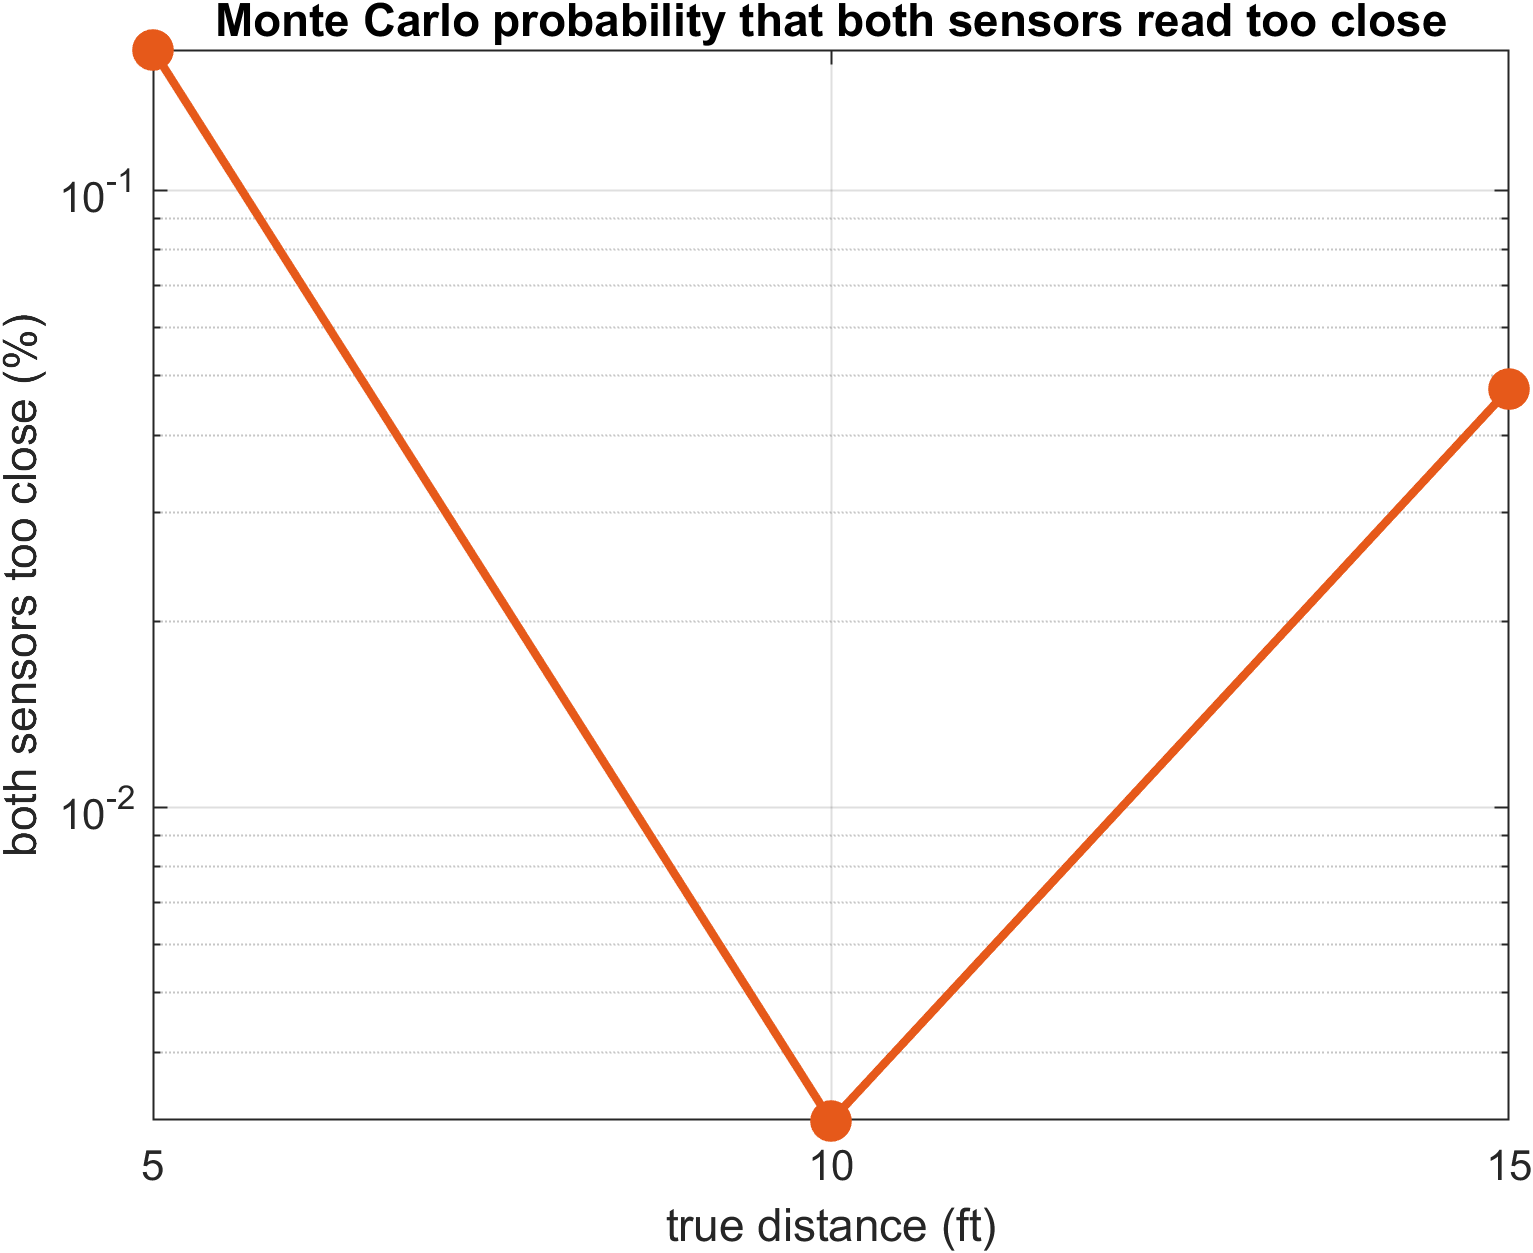
\includegraphics[width=0.98\linewidth,height=0.46\textheight,
                    keepaspectratio]{monte_carlo_results.png}%
            }{%
                \begin{tikzpicture}
                    \begin{semilogyaxis}[
                        width=\linewidth,
                        height=0.48\textheight,
                        xlabel={Distance (ft)},
                        ylabel={Both too close (\%)},
                        xtick={5,10,15},
                        ymin=0.001,
                        ymax=1,
                        grid=both,
                        tick label style={font=\scriptsize},
                        label style={font=\scriptsize}
                    ]
                        \addplot[color=vtorange,mark=*,very thick]
                            coordinates {(5,0.1687) (10,0.0031) (15,0.0476)};
                    \end{semilogyaxis}
                \end{tikzpicture}%
            }
        \end{column}
    \end{columns}
\end{frame}

\begin{frame}{Conclusions and recommendation}
    \begin{columns}[T,onlytextwidth]
        \begin{column}{0.54\textwidth}
            \textbf{Findings}
            \begin{itemize}
                \item Sensor 1 matches the true distance at 10 and 15 ft according to the t-tests.
                \item Sensor 2 matches the true distance only at 5 ft.
                \item Both-sensor early-reading events remain below 0.17\% at every distance.
            \end{itemize}
        \end{column}
        \begin{column}{0.42\textwidth}
            \begin{block}{Recommendation}
                Select \textbf{Sensor 1} for the autonomous vehicle. It provides better accuracy across the tested range and passes two of the three accuracy tests.
            \end{block}

            \vspace{0.25cm}
            \small Sensor 2 is slightly more precise at 5 and 15 ft, but overestimates distance at 10 and 15 ft.
        \end{column}
    \end{columns}
\end{frame}

\end{document}
